\chapter{TEST GENERATION}
\label{chapter:test_generation}

\section{Off-line Test Generation with Graphwalker}
\par
The user needs to have Java version 7 or 8 installed on the machine for test generation with Graphwalker. The off-line generation is supported via the command line interface, where the user needs to pass models and generation criteria as parameters to the Graphwalker \texttt{.jar} file. The user can generate tests from single as well as from multiple models simultaneously. The example usage is listed below.

\begin{lstlisting}
For single model:
java -jar graphwalker.jar offline -m Login.graphml random(edge_coverage(100))
\end{lstlisting}
\begin{lstlisting}
For multiple models:
java -jar graphwalker.jar offline 
-m src/test/resources/graphml/shared_state/Model_A.graphml random(edge_coverage(100)) 
-m src/test/resources/graphml/shared_state/Model_B.graphml random(edge_coverage(100))
-m src/test/resources/graphml/shared_state/Model_C.graphml random(edge_coverage(100))
-m src/test/resources/graphml/shared_state/Model_D.graphml random(edge_coverage(100))
\end{lstlisting}

\par
Graphwalker outputs the generated tests in form of a sequence of edges and vertexes. An example sequence can be observed in the listing below.

\begin{lstlisting}
e_Init
v_ClientNotRunning
e_StartClient
v_LoginPrompted
e_InvalidCredentials
v_LoginPrompted
e_ValidPremiumCredentials
v_Browse
e_Logout
\end{lstlisting}

\par
Graphwalker allows off-line test generation from models using multiple selection criteria. The general pattern for the test selection criteria can be observed in Figure \ref{Fig:raphwalker_testselection_example}.

\begin{figure} [htbp!]
\centering
					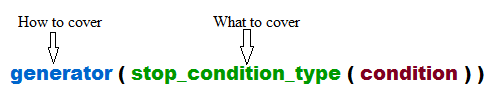
\includegraphics[width=1\textwidth]{figures/Graphwalker_testselection_example.png}
					\caption{\label{Fig:raphwalker_testselection_example} Graphwalker Test Selection pattern}
\end{figure}
\par
As the reader can observe, a selection criterion consists of a generator, a stop condition type and a condition. Generator stands for the coverage algorithm, which takes the stop condition type as a parameter. The stop condition type gives Graphwalker information about what exactly to cover using the coverage algorithm. The condition might vary depending on the stop condition type.

\subsection{Generator Algorithms}
\par
One of the generator algorithms in Graphwalker is called \texttt{random}, also known under the name Drunkard's walk or Random walk. This is the algorithm which will be used most extensively for the generation of tests in this thesis. This algorithm selects edges which are not blocked by guards, choosing one of them randomly and traversing it in order to reach the next vertex. This process is repeated until the stopping condition is met. Multiple stop conditions such as edge or vertex coverage can be used as parameters. Examples of the usage of this algorithm can be observed below. 
\begin{lstlisting}
random(vertex_coverage(100))
random(never)
random(reached_vertex(v_SomeVertex))
random(reached_vertex(v_SomeVertex) and edge_coverage(100))
random((reached_vertex(v_SomeVertex) and vertex_coverage(100)) || time_duration(500))
\end{lstlisting}

\par
The \texttt{weighted\_random} coverage works in the same way as the random algorithm, additionally it takes the weight annotations on edge labels into consideration and chooses the next edge based on them. Basically, the higher the edges weight, the more likely it is that Graphwalker will traverse that edge when its source vertex is reached. This is extremely useful when the company receives usage profiles for an application from customers, in order to test features with a higher usage more extensively. \texttt{weighted\_random} can be called in the same way as random, with the only change being the substitution of the algorithms name.

\par
\texttt{quick-random} tries to cover a model using the shortest path possible. It marks already taken edges as visited and tries not to traverse them again if another option is available. The problem is that it does not work with \acrshort{efsm} and might take an edge which is blocked by a guard. That is the reason why it cannot be used in our case, as most of the edges in our models are annotated with guards. As in the case of \texttt{weighted\_random} the algorithm can be called using the same syntax which is used for the random algorithm, by exchanging the functions name.  

\par
The \texttt{a\_Star} algorithm can be used to generate the shortest path to an edge or vertex in the model. In this case the passed stop condition needs to specify which edge or vertex needs to be reached, in order for the algorithm to terminate. The example usage can be found below.

\begin{lstlisting}
a_star(reached_edge(e_SomeEdge))
a_star(reached_vertex(v_SomeVertex))
\end{lstlisting}

\subsection{Stop Conditions}
\par
Edge and vertex coverage are the most used stop conditions for any type of random algorithm in Graphwalker. As an input parameter they take an integer which stands for the percentage that has to be covered. So, \texttt{random(edge\_coverage(95))} would mean that Graphwalker can stop only after it covers 95\% of the edges.

\par
The reached vertex or edge stop condition tells Graphwalker to stop the generation when a specific edge or vertex, passed to it as an argument, is reached while traversing the graph. For example, \texttt{a\_star(reached\_vertex(v\_SomeVertex))} would mean that traversal should stop when vertex with name \texttt{v\_SomeVertex} is reached.

\par
Other stop conditions are also available, such as \texttt{never} stopping the traversal, the \texttt{length} of the generated sequence, the \texttt{duration} of the traversal, dependency and requirement coverage, but none of them will be used in the scope of this thesis.

\section{Graphwalker GUI}
\par
To simplify the test generation even more, we decided to provide a \acrshort{gui} for off-line test generation, which is shown in Figure \ref{Fig:Graphwalker_GUi}.

\begin{figure} [htbp!]
	\centering
					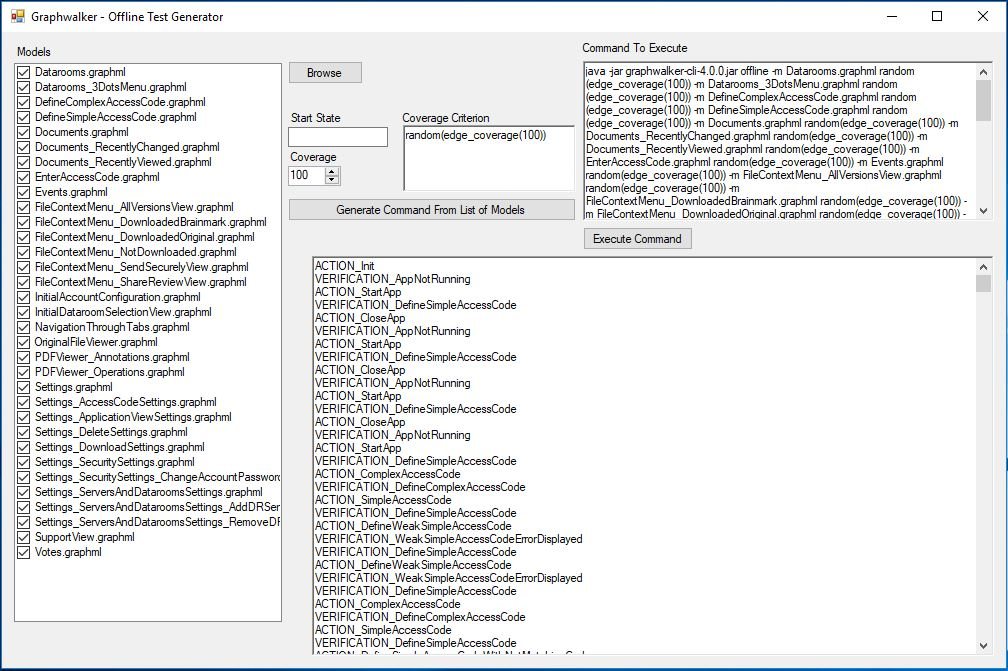
\includegraphics[width=0.95\textwidth]{figures/Graphwalker_GUI_screenshot}
					\caption{\label{Fig:Graphwalker_GUi} Graphwalker Off-line Test Generator}
\end{figure}

\par
The \acrshort{gui} is based on Windows Forms. The user needs to browse the folder where all the models and the graphwalker \texttt{.jar} file reside. Then they need to select the models to be included in the generation, as well as the coverage criterion. Unfortunately, for now it is only possible to generate commands which use one coverage criterion for all models, but the user has the possibility to alter the command inside the \textit{Command To Execute} text box, which makes it possible to add other criteria manually. After the resulting command is executed, it might contain duplicated states which are the result of Graphwalker switching from one model to another, which can happen when it reaches a shared state. The parsing of the whole document takes place as soon as raw output is generated, to remove these repeated references of a single state. As a result, Graphwalker generates parsed and well shaped results. It is worth mentioning that, after optimizing the solution, a sequence of states containing multiple millions of lines of states and transitions is getting parsed in roughly 10 seconds.

\section{Minimal Required Path}
\par
The generation of tests for all the 33 behavioral models, with 100\% random edge coverage and the parsing of the results, resulted in a sequence of 380,127 states and transitions. The roughly estimated time that was required to execute the test suite against \acrshort{aut} was 3,533 hours. This is not feasible for a company, as one test run would require 10 complete sprints (each taking 2 weeks) even if the automated tests were to be executed for 24 hours a day. This required changing the way tests where generated and compromising some test scenarios to reduce the size of the test sequence. For this reason we came up with the notion of \acrlong{mrp} (\acrshort{mrp}).

\par
\acrshort{mrp} stands for the shortest path needed to reach some state in a model from the base layer. It has the form of a Graphwalker test generation criterion composed of multiple models and the \texttt{a\_star} algorithm. Each model's description in the second layer contains the \acrshort{mrp}. An example for the Security Settings model's \acrshort{mrp} can be observed below.

\begin{lstlisting}
MRP: -m DefineSimpleAccessCode.graphml 
a_star(reached_vertex(v_InitialAccountConfiguration))
-m EnterAccessCode.graphml a_star(reached_vertex(v_DocumentsView))
-m Settings.graphml a_star(reached_vertex(v_SecuritySettings))
-m InitialAccountConfiguration.graphml 
a_star(reached_vertex(v_InitialDataroomSelectionView))
-m InitialDataroomSelectionView.graphml a_star(reached_vertex(v_DocumentsView)) 
-m NavigationThroughTabs.graphml a_star(reached_vertex(v_SettingsView))
\end{lstlisting}

After the \acrshort{mrp} is given to Graphwalker as a parameter, the user can add the current model with any coverage criterion. We decided to test \acrshort{bsc}'s base and navigation layers together with 100\% coverage of all the models contained in them and each model from the operations layer with 100\% coverage together with their \acrshort{mrp}. The test results are described in the next chapter.

